\documentclass[a4paper]{article}
\usepackage{amsmath}
\usepackage{amssymb}
\usepackage{graphicx}

\parindent=0em
\begin{document}
Q1\\\\
$\binom{n}{k}\ +\ \binom{n}{k+1}\\\\
=\dfrac{n!}{(n-k)!k!}\ +\ \dfrac{n!}{(n-k-1)!(k+1)!}\\
=\dfrac{n!}{(n-k-1)!k!(n-k)}\ +\ \dfrac{n!}{(n-k-1)!k!(k+1)}\\
=\dfrac{n!(k+1+n-k)}{(n-k-1)!k!(n-k)(k+1)}\\
=\dfrac{n!(n+1)}{(n-k)!(k+1)!}\\
=\dfrac{(n+1)!}{((n+1)-(k+1))!(k+1)!}\\\\
=\binom{n+1}{k+1}$\\
\\Q2\\
\\(a)\\
If we use each symbol once and only once among the 3 propositions ($\Pi(3,3)$), 2 operators ($\Pi(2,2)$), and 2 pairs of parentheses ($\binom{3}{2}$) given by the question:\\
Number of all wff's = $\Pi(3,3) * \Pi(2,2)* \binom{3}{2}\ =\ 24$\\ 
\\(b)\\
5 could be found:\\
$\{q\},\\ 
\{p \lor q\}, \\
\{p\land q\},\\
 \{\neg p\lor q\},\\
  \{\neg p \land q\}$\\
\\Q3\\
\\(a)\\
Let t = the expected time to leave the maze.\\
Under a uniform distribution, the 4 options share 1 probability equally, i.e. 0.25 probability each.\\
t = 0.25 * 5 + 0.25 * (3 + t) + 0.25 * 8 + 0.25 * (2 + t)\\
t = 1.25 + 0.75 + 0.25t + 2 + 0.5 + 0.25t\\
t = 4.5 + 0.5t\\
t = 9 (min)\\
\\(b)\\
This is different from (a) in that the wrong choice will not be taken again once already taken. Therefore, the probability will be uniformly distributed among only the remaining choices after 1 or 2 rounds of choice, i.e. 1/3 or 1/2.\\
$t = \dfrac{1}{4} * 5 +  \dfrac{1}{4} * 8\\ 
\hspace*{0.3cm} +  \dfrac{1}{4} * (3 + ( \dfrac{1}{3} * 5 +  \dfrac{1}{3} * 8 +  \dfrac{1}{3} * (2 +  \dfrac{1}{2} * 5 + \dfrac{1}{2} * 8)))\\
\hspace*{0.3cm} +  \dfrac{1}{4} * (2 + ( \dfrac{1}{3} * 5 +  \dfrac{1}{3} * 8 +  \dfrac{1}{3} * (3 + \dfrac{1}{2} * 5 + \dfrac{1}{2} * 8)))\\
\approx 8.167$ (min)\\
 \\Q4\\
\\(a)\\
Under a uniform distribution, when the point is at each vertex, moving left or right share equal probability(s) split from 1. Therefore, when it is at $v1$ and $v5$, it has only one choice which has 1 probability, and when it is at $v2-v4$, moving left or right share equal probabilityes, i.e. 0.5.\\  
$p_{1}(n+1) = \dfrac{1}{2}\ p_{2}(n)\\
p_{2}(n+1) = p_{1}(n) + \dfrac{1}{2}\ p_{3}(n)\\
p_{3}(n+1) = \dfrac{1}{2}\ p_{2}(n) + \dfrac{1}{2}\ p_{4}(n)\\
p_{4}(n+1) = \dfrac{1}{2}\ p_{3}(n) + p_{5}(n)\\
p_{5}(n+1) = \dfrac{1}{2}\ p_{4}(n)$\\
\\(b)\\
By solving the above equations on the basis of $p_{m}(n)=p_{m}(n+1)$ (m is the ordering of the vertex, $m \in [1,5], m \in \mathbb{N}) $ , the steady state probablities are:\\
$p_{1}(n) = p_{5}(n) = \dfrac{1}{8}\\\\
p_{2}(n) = p_{3}(n) = p_{4}(n) = \dfrac{1}{4}$\\\\
\\(c)\\
The mathematical expectation of the distance D to $v1$ at the stable status can be written as $$D = \sum_{m=1}^{5} p_{m}(n)\cdot (m-1)$$ in which m is the ordering of the vertex, $m \in [1,5], m \in \mathbb{N} $. When solved,\\
$$D = 2$$\\
Alternative solution: \\
At the stable status, the probabilities of $v1 ... v5$ are symmetric over $v3$.\\
$\therefore$ The expected distance to $v1$ is the distance between $v1$ and $v3$, which is 2.\\\\
\\Q5\\
\\(a)\\
For convenience, name the vertices as follows:\\\\
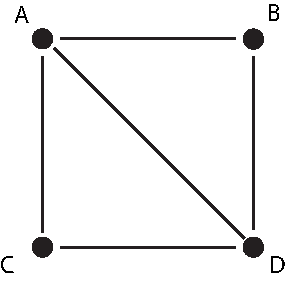
\includegraphics[scale=1]{fig1.pdf}\\\\
\{A, B, D\} and  \{A, C, D\} are cliques of chromatic number 3, and since each vertex connected by an edge must have different colors, in a valid 3-coloring pattern, B and C will have the same color, and 3 colors will be permutated over A, BC, D. \\
Ways of valid 3-coloring = $\Pi(3,3)\ =\ 6$\\
All ways of coloring: $3^{4}\ =\ 81$\\
$P(a)\ =\ \dfrac{6}{81}\ \approx\ 0.074$\\
\\(b)\\
Ways of valid 3-coloring = $\Pi(3,3)\ =\ 6$\\
Since there are 5 edges, all ways of coloring = $6^{5} =\ 7776$\\
$P(b)\ =\ \dfrac{6}{6^{5}}\ =\ \dfrac{1}{6^{4}}\ \approx 0.00077$
\end {document}


















